\documentclass{article}
\usepackage{polski}
\usepackage{blindtext}
\usepackage{amsmath}
\usepackage{mathtools}
\usepackage{graphicx} 
\usepackage{wrapfig}
\usepackage{amssymb}
\usepackage{multirow}
\usepackage[usenames,dvipsnames,svgnames,table]{xcolor}
\usepackage{float}
\usepackage[caption = false]{subfig}
\usepackage{caption}
\newcommand\tab[1][1cm]{\hspace*{#1}}
\usepackage[a4paper, left=2cm, right=2cm, top=2cm, bottom=2cm, headsep=1.2cm]{geometry}

\usepackage{titling}
\newcommand{\subtitle}[1]{%
  \posttitle{%
    \par\end{center}
    \begin{center}\large#1\end{center}
    \vskip0.5em}%
}


\begin{document}
\title{Szacowanie całek przy użyciu kwadratur Gaussa}
\author{Wiktoria Zaczyk}
\date{10.06.2020}

\maketitle

\begin{figure}[H]
\begin{center}

\includegraphics[height=0.3\linewidth]{agh.jpg}
\label{pierwszy} 
\end{center}
\end{figure}

\section{Wstęp teoretyczny}
\textbf{Całkowanie numeryczne}
\newline
Oznacza zastosowanie metod numerycznych w celu wyznaczenia przybliżonej wartości całki oznaczonej.Proste metody całkowania numerycznego polegają na przybliżeniu całki za pomocą odpowiedniej sumy ważonej wartości całkowanej funkcji w kilku punktach. Aby uzyskać dokładniejsze przybliżenie dzieli się przedział całkowania na niewielkie fragmenty. Ostateczny wynik jest sumą oszacowań całek w poszczególnych podprzedziałach.

\begin{equation}
\begin{array}{c}
C = \displaystyle \int_{a}^{b} f(x)dx 
\end{array}
\end{equation}

\newline
\setlength{\parindent}{0pt}
\textbf{Kwadratury Gaussa}
\newline
Rozpatrujemy kwadratury typu: 

\begin{equation}
\begin{array}{c}
S(f)=\displaystyle \sum^N_{k=0} A_k f(x_k)
\end{array}
\end{equation}

Współczynniki kwadratury z wagą p(x):
\begin{equation}
\begin{array}{c}
A_k = \displaystyle \int_{a}^{b} p(x)\Phi_k(x)dx 
\end{array}
\end{equation}

Numerycznie całkę policzyć można z następującego wzoru:

\begin{equation}
\begin{array}{c}
S(f)=\displaystyle \sum_{k=0 j}^N A_kf(x_k), \hspace{10} x\in[a,b]
\end{array}
\end{equation}

Ustalamy funkcję wagową $p(x)$
oraz liczbę węzłów $(N+1)$. Szukamy:
\begin{enumerate}
    \item położenia węzłów
    \item współczynników $A_k$
\end{enumerate}
tak aby rząd kwadratury był jak najwyższy.
Kwadratura tego typu nosi nazwę kwadratury
Gaussa. Do wyznaczenia kwadratur Gaussa
używa się wielomianów ortogonalnych.
\newline\newline
Ciąg wielomianów: $\{\varphi_n(x)\} = \{\varphi_0(x),...,\varphi_N(x)\}$ 
\newline 
Nazywamy ortogonalnymi w przedziale [a,b] jeśli
zachodzi pomiędzy nimi związek:

\begin{equation}
\begin{array}{c}
(\varphi_r, \varphi_s) = \displaystyle \int_{a}^{b} p(x) \varphi_r (x) \varphi_s (x)dx = 0 \hspace{15} r\ne s
\end{array}
\end{equation}

Tw.1. Wielomiany ortogonalne mają tylko pierwiastki rzeczywiste, leżące w przedziale $[a,b]$.
\newline\newline
Tw.2. Nie istnieje kwadratura Gaussa rzędu wyższego
niż $2(N+1)$. Kwadratura Gaussa jest rzędu $2(N+1)$
wtedy i tylko wtedy, gdy węzły $x_k$ są pierwiastkami
wielomianu $P_{N+1}(x)$.
\newline\newline
Tw. 3. Wszystkie współczynniki $A_k$
 w kwadraturach
Gaussa są dodatnie.
\newline\newline
Metoda kwadratur Gaussa jest zbieżna do każdej
funkcji ciągłej w $[a,b]$. Kwadratury te są dokładne dla
wielomianów stopnia $2N+1$
\newline\newline

\textbf{Kwadratury Gaussa-Legendre’a}
\newline
Posiada funkcję wagową postaci $p(x) = 1.$
Przybliża całkę oznaczoną z przedziału $[-1, 1]$. Współczynniki kwadratury można
wyznaczyć:

\begin{equation}
    A_k=-\frac{2}{(N+2)P_{N+2}(x_k)P_{N+1}(x_k)}
\end{equation}

By zastosować wzory z przedziału $[-1, 1]$ dla przedziału $[a, b]$ należy dokonać
transformacji liniowej zmiennej niezależnej. Wtedy przybliżenie całki ma postać:
 
 \begin{equation}
\begin{array}{c}
\displaystyle \int_{a}^{b} p(x)f(t)dt \approx S(f) = \frac{b-a}{2} \displaystyle \sum_{k=0 j}^N A_kf(t_k)
\end{array}
\end{equation}

dla $t_k=\frac{a+b}{2}+\frac{b-a}{2}x_k$ i węzłów rozłożonych w przedziale $[-1, 1]$. Węzłami są
pierwiastki n-tego wielomianu Legendre'a.

\vspace{5}
\setlength{\parindent}{0pt}
\textbf{Kwadratury Gaussa-Legendre’a}
\newline
Posiada funkcję wagową postaci $p(x) = e^{-x}$
Przybliża całkę oznaczoną z przedziału $[0, \infty]$. Współczynniki kwadratury można
wyznaczyć:

\begin{equation}
    A_k=\frac{((N+1)!)^2}{L_{N+2}(x_k)L_{N+1}(x_k)}
\end{equation}

Kwadratura z węzłami , które są zerami N-tego wielomianu Laguerre'a , ma postać:
 
 \begin{equation}
\begin{array}{c}
\displaystyle \int_{a}^{b} e^{-x}f(x)dx \approx S(f) = \displaystyle \sum_{k=0 j}^N A_kf(x_k)
\end{array}
\end{equation}


\setlength{\parindent}{-5pt}
\textbf{ Kwadratury Gaussa-Hermite’a}
\newline
Posiada funkcję wagową postaci $p(x) = e^{-x}$
Przybliża całkę oznaczoną z przedziału $[-\infty, \infty]$. Kwadratura z węzłami $x_k$, które są
zerami N-tego wielomianu Hermite'a $H_N(x)$ ma postać:
 
 \begin{equation}
\begin{array}{c}
\displaystyle \int_{a}^{b} e^{-x}f(x)dx \approx S(f) = \displaystyle \sum_{k=0 j}^N A_kf(x_k)
\end{array}
\end{equation}

Podczas sumowania każdej z kwadratur pomijamy wagę – ta jest uwzględniona we
współczynnikach $A_k$

\section{Cel zadania}

Zadaniem w trakcie laboratoriów było wyznaczyć wartości całki typu: 

\begin{enumerate}
    \item niewłaściwej metodą  kwadratury Gaussa-Legendre’a dla $a=10$ i liczby węzłów $n = 5, 6, 7, . . . , 70$ 
    
    \begin{equation}
        C_1=\displaystyle \int_{0}^{a}ln(x)dx=aln(a)-a
    \end{equation}
    
    \item przy użyciu kwadratury Gaussa-Laguerre’a oraz Gaussa-Legendre’a,
dla liczby węzłów $n = 5, 6, 7, . . . , 70$

    \begin{equation}
        C_2=\displaystyle \int_{0}^{\infty}(x-10)^2sin(4)e^{-x}dx
    \end{equation}
    
    \item przy użyciu kwadratury Gaussa-Hermite’a oraz Gaussa-Legendre’a, dla liczby węzłów $n = 5, 6, 7, . . . , 70$

    \begin{equation}
        C_3=\displaystyle \int_{-\infty}^{\infty}x^72^{-x^2+x+4)}e^{-x^2}dx
    \end{equation}

\end{enumerate}

\section{Wyniki}
\textbf{I.}

\begin{figure}[H]
\begin{center}
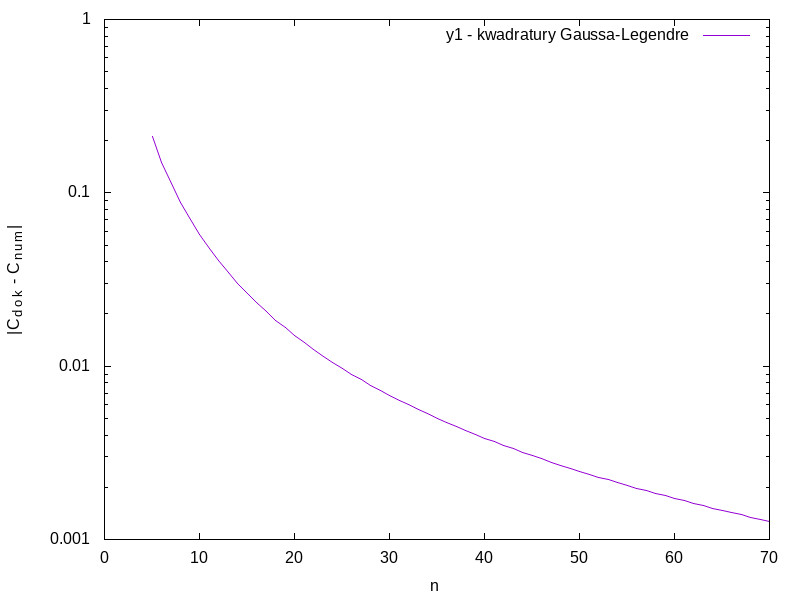
\includegraphics[height=0.5\linewidth]{zad1.jpg}
\caption{Wykres zależności modułu różnicy wartości dokładnej całki, a całki obliczonej numerycznie od ilości przyjętych
węzłów}
\label{pierwszy} 
\end{center}
\end{figure}

Jak można zauważyć na wykresie, wraz ze zwiększeniem liczby węzłów, cały czas
zwiększała się dokładność wyznaczonego przybliżenia wartości całki metodą
kwadratury Gaussa-Legendre’a.

\newpage
\textbf{II.}

\begin{figure}[H]
\begin{center}
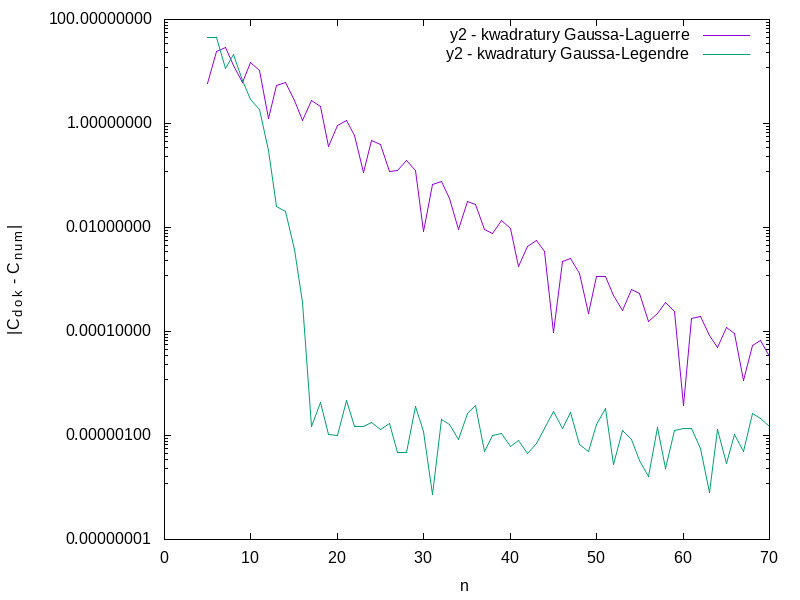
\includegraphics[height=0.5\linewidth]{zad2.jpg}
\caption{Wykres zależności modułu różnicy wartości dokładnej całki, a całki obliczonej numerycznie od ilości przyjętych
węzłów}
\label{pierwszy} 
\end{center}
\end{figure}
\newline
Dla metody kwadratur Gaussa-Legendre’a dokładność stale się zwiększała podczas
zwiększania liczby węzłów. Dla ich większej liczby następowały oscylacje różnicy
rozwiązania dokładnego z numerycznym i jakość wyznaczonego przybliżenia nie
zwiększała się znacznie. Dla metody kwadratur Gaussa-Laguerre’a mimo niewielkich oscylacji, jakość
przybliżenia zwiększała się przy zwiększaniu liczby węzłów do 70.
\newline
\textbf{III.}

\begin{figure}[H]
\begin{center}
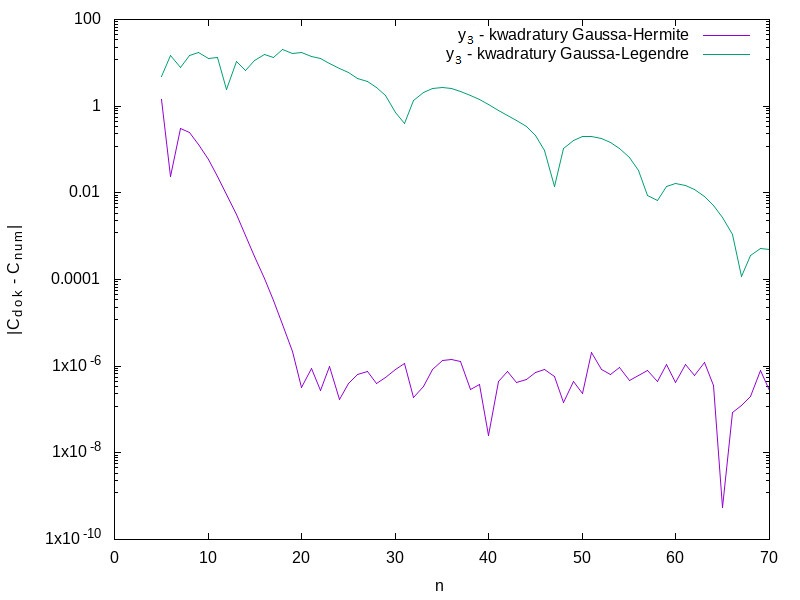
\includegraphics[height=0.5\linewidth]{zad3.jpg}
\caption{Wykres zależności modułu różnicy wartości dokładnej całki, a całki obliczonej numerycznie od ilości przyjętych
węzłów}
\label{pierwszy} 
\end{center}
\end{figure}

Dla metody kwadratur Gaussa-Hermite’a dokładność wyznaczonej wartości całki
oznaczonej III. zwiększała się podobnie jak dokładność przybliżenia całki II. metodą
kwadratur Gaussa-Legendre’a. Dla większej liczby przyjętych węzłów,
występowały oscylacje i dokładność nie zwiększała sie znacząco. Można zauważyć powtarzające się
'uskoki' wykresu, gdzie błąd przybliżenia najpierw rośnie, a następnie zaczyna maleć.
Dla całej dziedziny rozpatrywanej liczby węzłów, metoda kwadratur GaussaHermite’a pozwoliła mi uzyskać lepsze przybliżenie niż metoda kwadratur GaussaLegendre’a.

\textbf{I.}

\begin{figure}[H]
\begin{center}
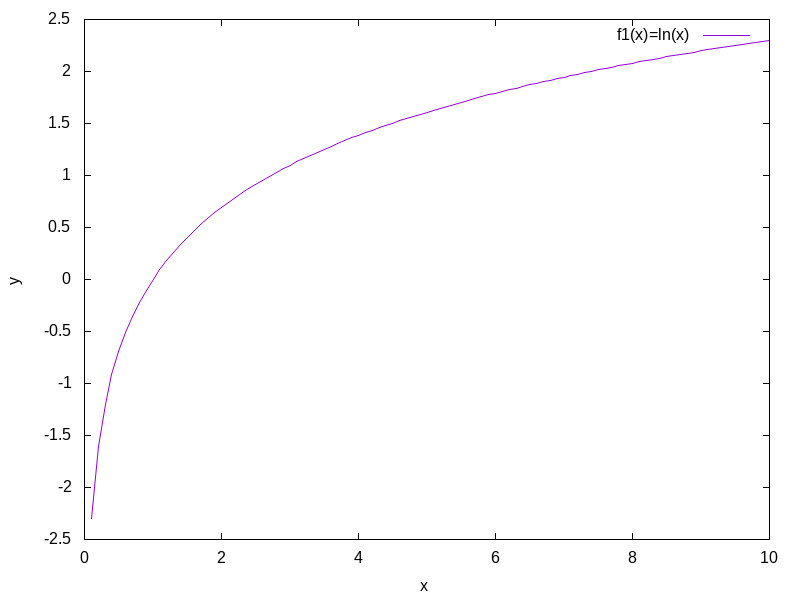
\includegraphics[height=0.5\linewidth]{f1.jpg}
\caption{Wykres iloczynu funkcji podcałkowej i funkcji wagowej$f(x)\cdot p(x)$}
\label{pierwszy} 
\end{center}
\end{figure}

\textbf{II.}

\begin{figure}[H]
\begin{center}
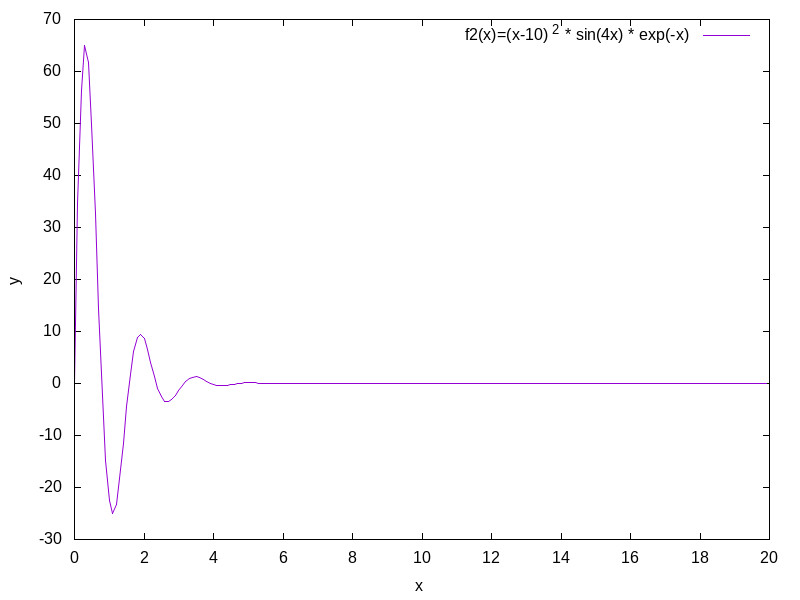
\includegraphics[height=0.5\linewidth]{f2.jpg}
\caption{Wykres iloczynu funkcji podcałkowej i funkcji wagowej$f(x)\cdot p(x)$}
\label{pierwszy} 
\end{center}
\end{figure}
\newpage
\textbf{III.}

\begin{figure}[H]
\begin{center}
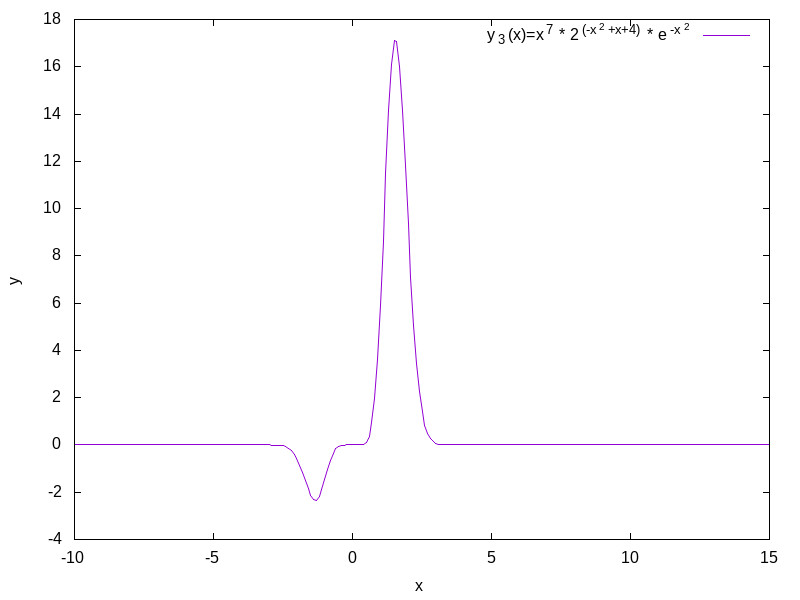
\includegraphics[height=0.5\linewidth]{f3.jpg}
\caption{Wykres iloczynu funkcji podcałkowej i funkcji wagowej$f(x)\cdot p(x)$}
\label{pierwszy} 
\end{center}
\end{figure}

W niektórych przypadkach
możliwe jest zastąpienie kwadratur Laguerre’a i Hermite’a kwadraturą Legendre’a; II. i III. Funkcja przyjmuje wartości bliskie zeru dla argumentów większych. Zatem zamiast liczyć całkę niewłaściwą, można ją obliczyć metodą kwadratur Legendre’a.

\section{Wnioski}
Dokładność zależy od liczby węzłów. Na wykresach iloczynu funkcji podcałkowej i funkcji wagowej widać, że wydajniej jest obliczyć przybliżoną wartość całki niż funkcji metodą Laguerre’a. Jeżeli pominąć funkcję wagową p(x), funkcja będzie oscylować i tłumić się dłużej. Uzyskane błędy przybliżenia są minimalnie większe od tych, uzyskanych metodą Simpsona, jednak
sama implementacja algorytmu, z wykorzystaniem biblioteki numerical recipes, jest dużo prostsza i pozwala na obliczenie niektórych całek niewłaściwychv metodą; prostą, wydajnaą i skuteczną.

\begin{thebibliography}{1}

\bibitem{1}
	Tomasz Chwiej, \emph{Całkowanie numeryczne przy użyciu kwadratur} \\
	\texttt{http://galaxy.agh.edu.pl/$\sim$chwiej/mn/calkowanie\_1819.pdf}	
\bibitem{2}	
	\texttt{https://pl.wikipedia.org/wiki/Całkowanie\_numeryczne}
	

\end{thebibliography}

\end{document}
